%!Tex Root = ../Arch_Linux_Installation.tex
% ./content_Arch_Linux_Installation/Packete
% ./content_Arch_Linux_Installation/Design
% ./content_Arch_Linux_Installation/Deklarationen
% ./content_Arch_Linux_Installation/Before_Installation
% ./content_Arch_Linux_Installation/After_Base_Installation

\section{Base Installation}

\begin{frame}[fragile]{Base Installation}{Keyboard Layout (for the Installation)}
  \begin{itemize}
    \item \inlinebox*{ls /usr/share/kbd/keymaps/**/*.map.gz | less}
    \begin{figure}
      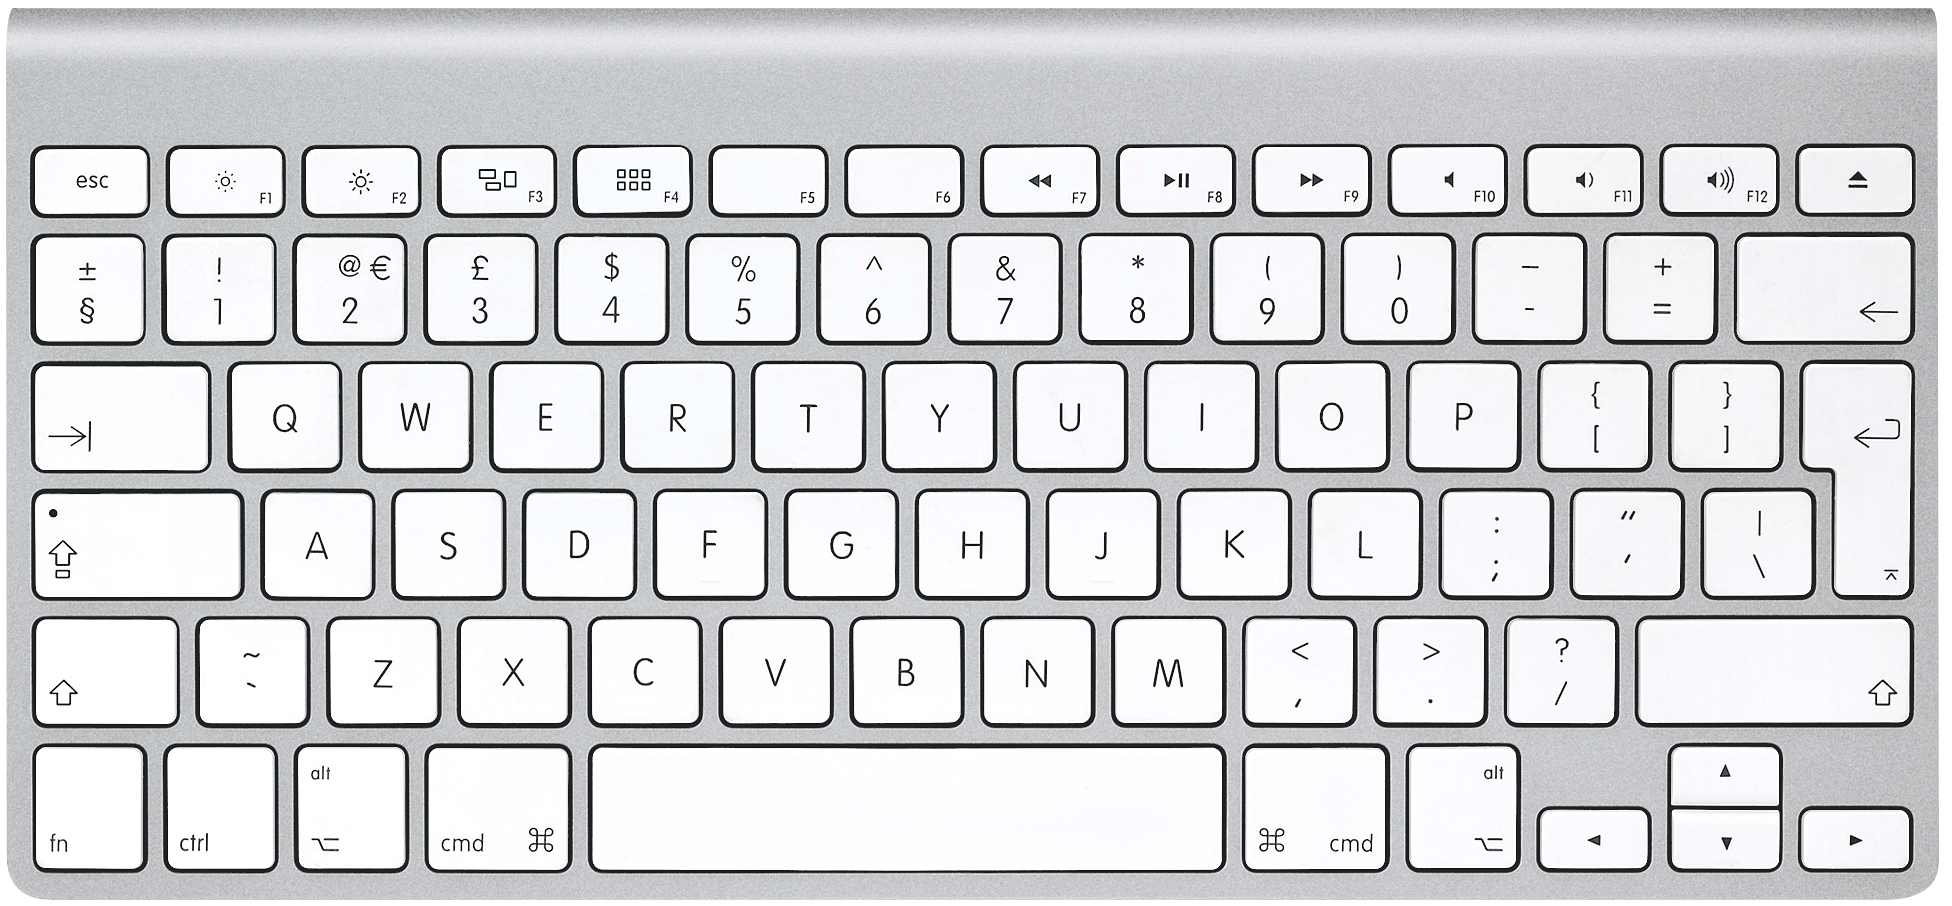
\includegraphics[width=0.5\textwidth]{./figures/keyboard.png}
    \end{figure}
    \item \inlinebox*{loadkeys de-latin1-nodeadkeys}
  \end{itemize}
\end{frame}

\begin{frame}[fragile]{Base Installation}{Wifi connection}
  \begin{itemize}
    \item \inlinebox*{ls /usr/share/kbd/keymaps/**/*.map.gz | less}
    \item \inlinebox*{ping -c 1 google.com}
    \item \inlinebox*{ip link or ip a (addr show)}
    \begin{Sidenote}
      \begin{itemize}
        \item sometimes one has to manually start the dhcp client `dhcpcd`
        \item netctl (and therefore wifi-menu) got removed from the Arch Linux ISO starting July 2020. To get connected while installing Arch, use `iwctl`. If it's blocked, either use that physical switch, or use `rfkill unblock wifi`. Then, type in `iwctl`. When you're in `iwctl`, use `device list` to see the name that the wifi router is using. For commands after this, replace device with the name of the device as found using the `device list` command. If you want to get the name of the network you want to use, use `station device scan` and then `station device get-networks`. After that, type in `station device connect SSID*`, with the *SSID being the name of the internet you want to use. If there is a password on the wifi, type that in when it asks for the wifi. After that, press Ctrl+C to get back to the terminal/root@archiso
      \end{itemize}
    \end{Sidenote}
  \end{itemize}
\end{frame}
